% !Rnw weave = knitr
% The Data
\section{Analyzing All Data}
\label{sec:overall}
Here we analyze all of the data.

First we load the data.
\begin{knitrout}
\definecolor{shadecolor}{rgb}{1, 1, 1}\color{fgcolor}\begin{kframe}
\begin{flushleft}
\ttfamily\noindent
\hlfunctioncall{require}\hlkeyword{(}\hlsymbol{useful}\hlkeyword{)}\hspace*{\fill}\\
\hlstd{}\hlfunctioncall{load}\hlkeyword{(}\hlstring{"{}C:/Users/Jared/week2/data/pakistan/pak.rdata"{}}\hlkeyword{)}\hspace*{\fill}\\
\hlstd{}\hlfunctioncall{corner}\hlkeyword{(}\hlsymbol{pak}\hlkeyword{,}{\ }\hlargument{c}{\ }\hlargument{=}{\ }\hlnumber{15}\hlkeyword{)}\mbox{}
\normalfont
\end{flushleft}
\begin{verbatim}
##   New_ID Age  Sex     Date Province District Tehsil        Village
## 1   1288  26 Male 29082010      KPK  Shangla Besham abaseen colony
## 2   1290  30 Male 29082010      KPK  Shangla Besham abaseen colony
## 3   1370  54 Male 28082010      KPK  Shangla Besham abaseen colony
## 4   1372  53 Male 28082010      KPK  Shangla Besham abaseen colony
## 5   1371  64 Male 28082010      KPK  Shangla Besham abaseen colony
##   Latitude Longitude Total Urban Rural
## 1    34.94     72.88  90.6     -  90.6
## 2    34.94     72.88  90.6     -  90.6
## 3    34.94     72.88  90.6     -  90.6
## 4    34.94     72.88  90.6     -  90.6
## 5    34.94     72.88  90.6     -  90.6
##                                 Accommodation StagnantWater
## 1 Collective centers (school/Public building)           Few
## 2                                 Host family           Few
## 3          On the site of the house (Damaged)           Few
## 4          On the site of the house (Damaged)          None
## 5          On the site of the house (Damaged)          None
\end{verbatim}
\end{kframe}
\end{knitrout}



Now we build a distribution and visualize it in Figure ~\ref{fig:allDist}.
\begin{figure}[!hbtp]
\begin{knitrout}
\definecolor{shadecolor}{rgb}{1, 1, 1}\color{fgcolor}\begin{kframe}
\begin{flushleft}
\ttfamily\noindent
\hlfunctioncall{source}\hlkeyword{(}\hlstring{"{}C:/Users/Jared/week2/R/distFuncs.r"{}}\hlkeyword{)}\hspace*{\fill}\\
\hlstd{}\hlsymbol{ricePerc}{\ }\hlassignement{\usebox{\hlnormalsizeboxlessthan}-}{\ }\hlfunctioncall{build.dist}\hlkeyword{(}\hlargument{data}{\ }\hlargument{=}{\ }\hlsymbol{pak}\hlkeyword{,}{\ }\hlargument{lhs}{\ }\hlargument{=}{\ }\hlstring{"{}New\usebox{\hlnormalsizeboxunderscore}ID"{}}\hlkeyword{,}{\ }\hlargument{group}{\ }\hlargument{=}{\ }\hlstring{"{}Province"{}}\hlkeyword{,}\hspace*{\fill}\\
\hlstd{}{\ }{\ }{\ }{\ }\hlargument{question}{\ }\hlargument{=}{\ }\hlstring{"{}RiceLost"{}}\hlkeyword{)}\hspace*{\fill}\\
\hlstd{}\hlsymbol{ricePerc}\hlkeyword{\usebox{\hlnormalsizeboxdollar}}\hlsymbol{Size}{\ }\hlassignement{\usebox{\hlnormalsizeboxlessthan}-}{\ }\hlstring{"{}All"{}}\hspace*{\fill}\\
\hlstd{}\hlfunctioncall{ggplot}\hlkeyword{(}\hlsymbol{ricePerc}\hlkeyword{,}{\ }\hlfunctioncall{aes}\hlkeyword{(}\hlargument{x}{\ }\hlargument{=}{\ }\hlsymbol{RiceLost}\hlkeyword{,}{\ }\hlargument{y}{\ }\hlargument{=}{\ }\hlsymbol{Percent}\hlkeyword{)}\hlkeyword{)}{\ }\hlkeyword{+}{\ }\hlfunctioncall{geom\usebox{\hlnormalsizeboxunderscore}bar}\hlkeyword{(}\hlargument{stat}{\ }\hlargument{=}{\ }\hlstring{"{}identity"{}}\hlkeyword{)}{\ }\hlkeyword{+}\hspace*{\fill}\\
\hlstd{}{\ }{\ }{\ }{\ }\hlfunctioncall{facet\usebox{\hlnormalsizeboxunderscore}wrap}\hlkeyword{(}\hlkeyword{\urltilda{}}\hlsymbol{Province}\hlkeyword{)}{\ }\hlkeyword{+}{\ }\hlfunctioncall{opts}\hlkeyword{(}\hlargument{axis.text.x}{\ }\hlargument{=}{\ }\hlfunctioncall{theme\usebox{\hlnormalsizeboxunderscore}text}\hlkeyword{(}\hlargument{angle}{\ }\hlargument{=}{\ }\hlnumber{90}\hlkeyword{)}\hlkeyword{)}\mbox{}
\normalfont
\end{flushleft}
\end{kframe}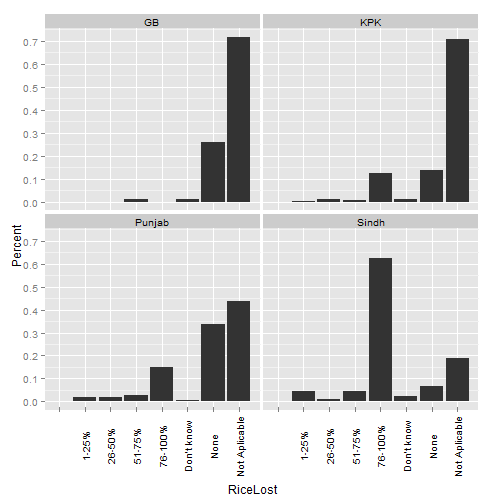
\includegraphics[width=.9\linewidth]{writeup/overall/figuresoverallDist} 
\end{knitrout}

\caption{Graphical view of the distribution of responses for all the data.\label{fig:allDist}}
\end{figure}

Quick comparison using just 5 Tehsils per province.
\begin{figure}[!hbtp]
\begin{knitrout}
\definecolor{shadecolor}{rgb}{1, 1, 1}\color{fgcolor}\begin{kframe}
\begin{flushleft}
\ttfamily\noindent
\hlsymbol{pak5}{\ }\hlassignement{\usebox{\hlnormalsizeboxlessthan}-}{\ }\hlsymbol{pak}\hlkeyword{[}\hlsymbol{pak}\hlkeyword{\usebox{\hlnormalsizeboxdollar}}\hlsymbol{Tehsil}{\ }\hlkeyword{\usebox{\hlnormalsizeboxpercent}in\usebox{\hlnormalsizeboxpercent}}{\ }\hlfunctioncall{unlist}\hlkeyword{(}\hlfunctioncall{dlply}\hlkeyword{(}\hlsymbol{pak}\hlkeyword{,}{\ }\hlargument{.variables}{\ }\hlargument{=}{\ }\hlstring{"{}Province"{}}\hlkeyword{,}\hspace*{\fill}\\
\hlstd{}{\ }{\ }{\ }{\ }\hlargument{.fun}{\ }\hlargument{=}{\ }\hlsymbol{village.list}\hlkeyword{,}{\ }\hlargument{num}{\ }\hlargument{=}{\ }\hlnumber{5}\hlkeyword{,}{\ }\hlargument{unit}{\ }\hlargument{=}{\ }\hlstring{"{}Tehsil"{}}\hlkeyword{)}\hlkeyword{)}\hlkeyword{,}{\ }\hlkeyword{]}\hspace*{\fill}\\
\hlstd{}\hlsymbol{pak5}\hlkeyword{\usebox{\hlnormalsizeboxdollar}}\hlsymbol{Tehsil}{\ }\hlassignement{\usebox{\hlnormalsizeboxlessthan}-}{\ }\hlfunctioncall{factor}\hlkeyword{(}\hlsymbol{pak5}\hlkeyword{\usebox{\hlnormalsizeboxdollar}}\hlsymbol{Tehsil}\hlkeyword{)}\hspace*{\fill}\\
\hlstd{}\hlsymbol{rice5Perc}{\ }\hlassignement{\usebox{\hlnormalsizeboxlessthan}-}{\ }\hlfunctioncall{build.dist}\hlkeyword{(}\hlargument{data}{\ }\hlargument{=}{\ }\hlsymbol{pak5}\hlkeyword{,}{\ }\hlargument{lhs}{\ }\hlargument{=}{\ }\hlstring{"{}New\usebox{\hlnormalsizeboxunderscore}ID"{}}\hlkeyword{,}{\ }\hlargument{group}{\ }\hlargument{=}{\ }\hlstring{"{}Province"{}}\hlkeyword{,}\hspace*{\fill}\\
\hlstd{}{\ }{\ }{\ }{\ }\hlargument{question}{\ }\hlargument{=}{\ }\hlstring{"{}RiceLost"{}}\hlkeyword{)}\hspace*{\fill}\\
\hlstd{}\hlsymbol{rice5Perc}\hlkeyword{\usebox{\hlnormalsizeboxdollar}}\hlsymbol{Size}{\ }\hlassignement{\usebox{\hlnormalsizeboxlessthan}-}{\ }\hlstring{"{}5"{}}\hspace*{\fill}\\
\hlstd{}\hlsymbol{compare5}{\ }\hlassignement{\usebox{\hlnormalsizeboxlessthan}-}{\ }\hlfunctioncall{compare.dist}\hlkeyword{(}\hlsymbol{ricePerc}\hlkeyword{,}{\ }\hlsymbol{rice5Perc}\hlkeyword{,}{\ }\hlargument{by}{\ }\hlargument{=}{\ }\hlfunctioncall{c}\hlkeyword{(}\hlstring{"{}Province"{}}\hlkeyword{,}\hspace*{\fill}\\
\hlstd{}{\ }{\ }{\ }{\ }\hlstring{"{}RiceLost"{}}\hlkeyword{)}\hlkeyword{)}\hspace*{\fill}\\
\hlstd{}\hlsymbol{compare5}\hlkeyword{\usebox{\hlnormalsizeboxdollar}}\hlsymbol{Partial.Size}{\ }\hlassignement{\usebox{\hlnormalsizeboxlessthan}-}{\ }\hlfunctioncall{impute.col}\hlkeyword{(}\hlargument{col}{\ }\hlargument{=}{\ }\hlsymbol{compare5}\hlkeyword{\usebox{\hlnormalsizeboxdollar}}\hlsymbol{Partial.Size}\hlkeyword{,}\hspace*{\fill}\\
\hlstd{}{\ }{\ }{\ }{\ }\hlnumber{5}\hlkeyword{)}\hspace*{\fill}\\
\hlstd{}\hlfunctioncall{ggplot}\hlkeyword{(}\hlsymbol{rice5Perc}\hlkeyword{,}{\ }\hlfunctioncall{aes}\hlkeyword{(}\hlargument{x}{\ }\hlargument{=}{\ }\hlsymbol{RiceLost}\hlkeyword{,}{\ }\hlargument{y}{\ }\hlargument{=}{\ }\hlsymbol{Percent}\hlkeyword{)}\hlkeyword{)}{\ }\hlkeyword{+}{\ }\hlfunctioncall{geom\usebox{\hlnormalsizeboxunderscore}bar}\hlkeyword{(}\hlargument{stat}{\ }\hlargument{=}{\ }\hlstring{"{}identity"{}}\hlkeyword{)}{\ }\hlkeyword{+}\hspace*{\fill}\\
\hlstd{}{\ }{\ }{\ }{\ }\hlfunctioncall{facet\usebox{\hlnormalsizeboxunderscore}wrap}\hlkeyword{(}\hlkeyword{\urltilda{}}\hlsymbol{Province}\hlkeyword{)}{\ }\hlkeyword{+}{\ }\hlfunctioncall{opts}\hlkeyword{(}\hlargument{axis.text.x}{\ }\hlargument{=}{\ }\hlfunctioncall{theme\usebox{\hlnormalsizeboxunderscore}text}\hlkeyword{(}\hlargument{angle}{\ }\hlargument{=}{\ }\hlnumber{90}\hlkeyword{)}\hlkeyword{)}\mbox{}
\normalfont
\end{flushleft}
\end{kframe}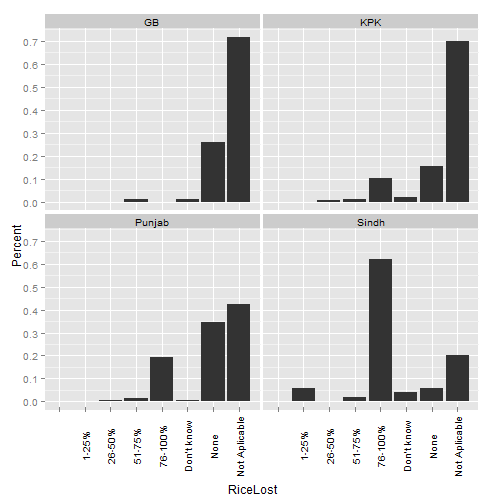
\includegraphics[width=.9\linewidth]{writeup/overall/figuresfiveDist} 
\end{knitrout}

\caption{Distribution for five villages per tehsil.\label{fig:fiveDist}}
\end{figure}
